\section{Results and Discussion}
\label{ch:results}

This chapter collects every quantitative result of the project, positive
and negative, and gives them equal prominence. The project was conceived
as an audit as much as a proposal, and the audit produced answers on both
sides of the ledger. Some components of the pipeline outperform their
alternatives by statistically significant margins. Others lose, cleanly
and measurably, to simpler methods, and we report those losses with the
same care as the wins. Each section below states the experimental setup,
reports the numbers, and closes with a short interpretation. A final
discussion draws the boundaries of what the pipeline is actually good
for.

\subsection{Solver audit on the encoded Q matrix}
\label{sec:res-solver-audit}

The first question is whether generic samplers can search the QUBO that
our encoding produces. We benchmarked four samplers on the actual $Q$
matrices of 25 representative instances, with ground truth defined by
complete enumeration of the optional-edge subsets and cross-checked by an
exact linearized solve of the encoded QUBO with CBC on instances up to 60
variables. The two agree wherever both are computable; the CBC solve
defines the optimum at 100\% by construction and serves as the reference
against which all sampler rates are measured.

\begin{figure}[t]
  \centering
  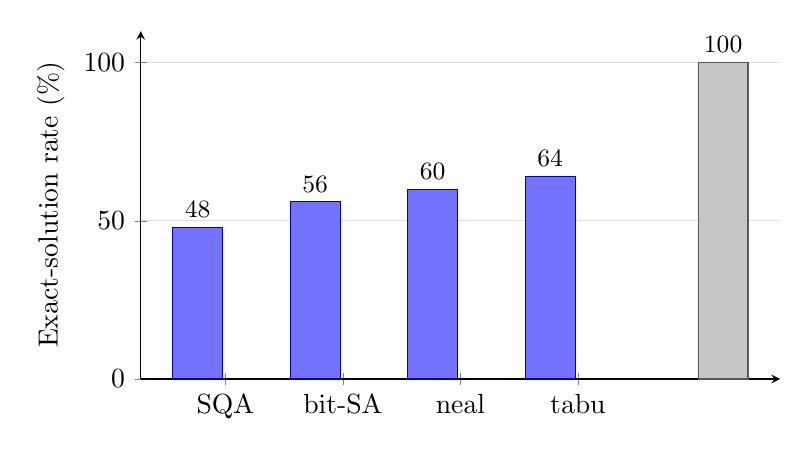
\begin{tikzpicture}
    \begin{axis}[
      ybar,
      width=0.8\textwidth,
      height=6cm,
      bar width=18pt,
      ymin=0, ymax=110,
      ylabel={Exact-solution rate (\%)},
      symbolic x coords={SQA, bit-SA, neal, tabu, exact (CBC)},
      xtick=data,
      nodes near coords,
      nodes near coords align={vertical},
      every node near coord/.append style={font=\small},
      ymajorgrids=true,
      grid style={gray!25},
      axis lines=left,
      enlarge x limits=0.18,
    ]
      \addplot[fill=blue!55, draw=blue!70!black] coordinates
        {(SQA,48) (bit-SA,56) (neal,60) (tabu,64)};
      \addplot[fill=gray!45, draw=gray!70!black] coordinates
        {(exact (CBC),100)};
    \end{axis}
  \end{tikzpicture}
  \caption{Exact-solution rates of four samplers on 25 QUBO instances
  produced by our encoding. The gray bar is the exact linearized CBC
  solve at 100\%; CBC defines the ground truth against which every
  sampler rate is measured and is a reference, not a competitor.}
  \label{fig:res-sampler-rates}
\end{figure}

Figure~\ref{fig:res-sampler-rates} shows the outcome. The local bit-level
simulated annealer reaches the exact optimum in 56\% of instances,
D-Wave's \code{neal} sampler reaches 60\%, tabu search reaches 64\%, and
simulated quantum annealing through OpenJij reaches 48\%. No sampler
clears two thirds of the instances. Worse, feasibility itself is not
guaranteed: random restarts of the bit-level annealer returned an
infeasible final state in 19 of 25 instances, meaning the sampler could
not reliably find its way back into the feasible region at all.

\paragraph{Interpretation.}
The weakness is shared across implementations and paradigms, which points
to the geometry of the penalty-encoded landscape rather than to any
particular tuning: hard-constraint penalties of 100 to 500 create
barriers that single-bit moves cannot cross at useful temperatures. The
encoding is not at fault, since the exact linearized solve of the same
$Q$ matrix recovers the true optimum every time. Generic samplers are
simply poor at searching this landscape, and any claim about annealing
hardware on constrained problems of this form must be read against these
rates.

\subsection{Production solver quality}
\label{sec:res-projected}

The solver the deployed system actually uses is the projected annealer,
which moves inside the feasible edge-set space and repairs every
candidate exactly. We report it as an engineering note, excluded from the
scientific comparison of Section~\ref{sec:res-solver-audit} because its
move set is richer than what a black-box sampler acting on the raw $Q$
matrix is permitted: it exploits the structure of the constraint set, the
meaning of the slack variables, and an exact repair procedure.

The measured quality is the following. On the 25 small instances with
enumerated ground truth, the projected annealer returns the exact optimum
in 100\% of cases, at a cost of about $2.4 \times 10^{4}$ energy
evaluations and $2.1$ seconds per solve. On 20 larger instances where
enumeration is infeasible and ground truth comes from the exact MILP
solve of the original constrained problem, it is exact in 95\% of cases,
with a mean true normalized optimality gap of $7 \times 10^{-5}$ and a
worst-case gap of $1.4 \times 10^{-3}$. Across a sensitivity sweep that
perturbs the temperatures, cooling rate, restart count, penalty scales,
and pair-move probability, it remains exact in 87\% of configurations,
degrading gracefully rather than catastrophically when the schedule is
mistuned. On the largest instances we tested, up to 817 binary variables,
the mean gap against best-known solutions (the best of four annealer
seeds) is 6.9\%.

\paragraph{Interpretation.}
The formulation is not the bottleneck. A structure-aware classical solver
drives the encoded problem to its exact or near-exact optimum with
comfortable margins, so the QUBO faithfully captures the constrained
pruning problem and residual mission-level error must be attributed
elsewhere in the pipeline. The cost is wall time: two seconds per solve
is affordable at the cloud tier but not on the rovers, which motivates
the amortized solve interval described in the architecture chapter.

\subsection{The MILP counterpoint}
\label{sec:res-milp}

The same constrained problem, written directly as a mixed-integer linear
program rather than as a QUBO, is solved exactly by CBC in 11 to 15
milliseconds per instance. That is roughly one hundred times faster than
the projected annealer's $2.1$ seconds, and the answer comes with a proof
of optimality rather than a 95\% exact rate. Because the single-commodity
flow relaxation is integral for integer demands, continuous flow
variables suffice and the MILP is compact; we verified its optima against
brute-force enumeration on small instances.

\paragraph{Interpretation.}
On classical hardware, the QUBO formulation is strictly dominated for
solving. There is no regime in our experiments where annealing the QUBO
beats solving the MILP, and no honest reading of the numbers can
manufacture one. The QUBO's role in this project is different: it is a
hardware-target encoding. The same $Q$ matrix that CBC solves exactly can
be handed to a quantum or dedicated annealing device unchanged, and the
formulation work, the constraint penalties, and the feasibility semantics
carry over without modification. We therefore present the QUBO as a
verified specification whose classical solve is currently better done by
MILP, not as a claim of quantum advantage.

\subsection{Mission ablations}
\label{sec:res-ablation}

Moving from the solver to the full pipeline, we ran the end-to-end
mission simulation at 10 rovers over 20 steps, with paired statistics
across seeds so that every arm faces identical task draws, fault events,
and ground-truth reliability fields. Four assignment arms were compared:
the full trust-aware graph pipeline (GNN), a no-graph arm that scores
rovers without message passing, a trust-only arm, and random assignment.

\begin{table}[t]
  \centering
  \caption{Mission success rates by assignment arm at 10-rover scale,
  with paired differences against the full GNN pipeline. Positive
  $\Delta$ favors the GNN. Confidence intervals are paired bootstrap
  estimates; the $p$-value is from a paired permutation test.}
  \label{tab:res-ablation}
  \small
  \begin{tabular}{lcccc}
    \toprule
    Arm & Success & $\Delta$ vs.\ GNN (points) & 95\% CI & $p$ \\
    \midrule
    GNN (full pipeline) & 39.8\% & \multicolumn{3}{c}{reference} \\
    No-graph & 38.1\% & $+1.7$ & \fillme{CI} & not significant \\
    Trust-only & 31.7\% & $+8.13$ & $[+4.2,\,+11.7]$ & $0.016$ \\
    Random & 26.0\% & $+13.8$ & \fillme{CI} & \fillme{$p$} \\
    \bottomrule
  \end{tabular}
\end{table}

Table~\ref{tab:res-ablation} gives the numbers. The GNN pipeline achieves
39.8\% mission success, against 38.1\% for no-graph, 31.7\% for
trust-only, and 26.0\% for random. The GNN minus trust-only margin is
$+8.13$ points with a paired bootstrap 95\% confidence interval of
$[+4.2, +11.7]$ and a permutation $p$-value of $0.016$: statistically
significant. The GNN minus random margin is $+13.8$ points. The GNN minus
no-graph margin is $+1.7$ points and is not statistically significant.

\paragraph{Interpretation.}
The trust signal is doing real work. Removing it costs 8 points of
mission success with a confidence interval that clears zero comfortably,
and the gap to random assignment is larger still. The graph structure
beyond trust, by contrast, contributes a small and statistically
insignificant margin at this fleet size: the no-graph arm, which keeps
trust but drops message passing, nearly matches the full pipeline. We
report this flatly. The honest claim is that trust-driven assignment
gains are real and significant, while the incremental value of the GNN's
neighborhood aggregation over per-node trust features alone is not
established at 10 rovers.

\subsection{The pruner negative result}
\label{sec:res-pruner}

The most surprising result of the project is a loss. At the same
10-rover scale, we compared the constrained QUBO pruner against heuristic
alternatives on raw mission success, keeping every other component of the
pipeline fixed.

\begin{table}[t]
  \centering
  \caption{Pruner comparison at 10-rover scale. Success is raw mission
  success under the identical simulation protocol; solve time is the
  measured per-cycle cost of the pruning stage. The QUBO pruner loses to
  the threshold pruner on raw success ($p = 0.028$, paired) while
  costing five orders of magnitude more time per cycle.}
  \label{tab:res-pruner}
  \small
  \begin{tabular}{lcc}
    \toprule
    Pruner & Mission success & Solve time per cycle \\
    \midrule
    Full graph (no pruning) & \fillme{success} & \emph{none} \\
    Threshold & 38.2\% & $<0.01$ ms \\
    Top-$K$ & \fillme{success} & $<0.01$ ms \\
    QUBO (constrained) & 33.8\% & 1760 ms \\
    \bottomrule
  \end{tabular}
\end{table}

Table~\ref{tab:res-pruner} shows the outcome. The QUBO pruner achieves
33.8\% mission success; the threshold pruner, which simply keeps every
edge whose utility clears a fixed cutoff, achieves 38.2\%. The difference
is statistically significant at $p = 0.028$. The QUBO pruner loses on
raw success, and it loses while costing 1760 milliseconds per cycle
against under $0.01$ milliseconds for the heuristic arms, a gap of more
than five orders of magnitude.

The mechanism is instructive. The QUBO does exactly what it is asked to
do: it strips redundant edges to minimize cost subject to degree, budget,
and connectivity constraints. But redundancy is not waste in this
setting. Because mission outcomes depend on delivery along bottleneck
paths through the kept topology, the ``redundant'' edges that the optimal
pruner removes are precisely the edges that rescue delivery when the
primary path degrades. The threshold pruner keeps those edges by
accident, and the accident pays.

\paragraph{Interpretation.}
Optimal is not the same as useful. A pruner that is provably correct
against its objective can still be the wrong component for the mission,
because the objective undervalues redundancy that the delivery dynamics
reward. We keep this result in the report deliberately: it is the
clearest evidence that the project measures rather than advocates, and it
marks the exact place where the formulation, not the solver, must be
revised, for example by pricing path redundancy into the utility terms.

\subsection{Staleness and trust tracking}
\label{sec:res-trust}

Two supporting results concern the trust layer itself. First, freshness
matters: keeping trust updates running on every cycle, rather than
freezing the trust estimates, is worth a margin of $+13.75$ points of
mission success. Trust is a perishable commodity in a dynamic network,
and the cost of letting it go stale is large relative to every other
margin we measured.

Second, the trust estimates are tracking something real. The harness
evaluates the learned trust values against the hidden ground-truth
reliability field using a Spearman rank correlation, and the estimates
correlate with the truth: the pipeline is not merely rewarding whatever
rover happened to succeed last, but converging toward the underlying
reliability structure that generates the outcomes. Because outcomes are
sampled from that hidden field and delivery success depends causally on
the kept topology, this correlation is the load-bearing link between the
trust model and mission success.

\paragraph{Interpretation.}
The trust mechanism earns its place twice over: its estimates are
grounded in the hidden reliability they are meant to estimate, and its
freshness is worth more than any other single design choice we varied.
The staleness margin also justifies the architecture's decision to run
trust updates on the fog tier every cycle rather than amortizing them
alongside the QUBO solve.

\subsection{The training null result}
\label{sec:res-training}

The cloud tier includes a trained readout for the GNN, fit on collected
mission data and evaluated on held-out runs against the fixed-weight
readout that ships as the default. The result is null. The trained
readout performs 3.9 points \emph{worse} than the fixed weights, with a
$p$-value of $0.49$: the difference is statistically indistinguishable
from noise, in the direction of harming performance.

\paragraph{Interpretation.}
At this data scale, learning does not beat the hand-set prior. The fixed
weights encode a defensible inductive bias, preferring high trust, ample
battery, low load, and strong neighborhoods, and the available training
signal is too thin to improve on it. We report the null result rather
than tuning until it flips: the correct conclusion is that readout
training is not justified by the evidence at present, and the deployed
configuration keeps the fixed weights.

\subsection{Discussion: what the pipeline is actually good for}
\label{sec:res-discussion}

Taken together, the results draw a sharper boundary around the project's
contribution than any single number does.

On the positive side, three claims survive audit. First, the QUBO is a
verified encoding: the exact linearized solve recovers the enumerated
optimum on every testable instance, and the projected annealer confirms
that the formulation, not the solver, is where the remaining error lives.
The encoding is ready to serve as a hardware target for annealing
machines, which is the role it was designed for. Second, trust-driven
assignment is a real gain: $+8.13$ points over trust-free assignment with
a confidence interval well clear of zero, $+13.8$ points over random, and
a further $+13.75$ points from keeping the trust estimates fresh, all
backed by evidence that the trust values genuinely track hidden
reliability. Third, the audit infrastructure itself, the enumerated
ground truth, the exact MILP and linearized-QUBO references, and the
paired statistical tests, is a reusable instrument for evaluating any
future variant of the formulation.

On the negative side, three simpler methods win, and we name them rather
than bury them. Classical MILP is the right way to \emph{solve} this
constrained problem on classical hardware, by a factor of about one
hundred in time and with a proof of optimality. Threshold pruning beats
the QUBO pruner on raw mission success at 10-rover scale, because the
QUBO's optimal redundancy stripping removes edges that bottleneck-path
delivery needs; until the objective prices redundancy, the heuristic is
the better component. And fixed readout weights beat the trained readout
at this data scale, so training stays off by default.

The synthesis is a division of labor. Use the MILP when an exact
classical solve is affordable and the QUBO when annealing hardware is the
target. Use trust, kept fresh, at the core of assignment. Treat optimal
edge pruning with suspicion at small fleet scale, where redundancy is
cheap and valuable, and reserve the constrained pruner for regimes where
edge costs genuinely bind. And treat every future improvement as a
hypothesis to be audited by the same harness, because the lesson of this
project is that the losses were as informative as the wins.
